\HeaderQuote{tmp}{tmp} 

\chapter{Generating Training Data}\label{ch:gentrdat} 

For \jsp\ there are $N_{\text{train}}$ problem instances generated using $n$ 
jobs and $m$ machines for processing times, $\vec{p}$, following the same data 
distribution and a random $\vsigma$ permutations, summarised in 
\cref{tbl:features}.  

\subsection{\Jsp\ tree representation}\label{sec:gen:gametree}
When building a complete \jsp\ schedule, $K=n\cdot m$ dispatches must be 
made sequentially.
A job is placed at the earliest available time slot for its next machine, 
whilst still fulfilling constraints \cref{eq:permutation,eq:oneJobPerMac}.
%that each machine can handle at most one job at each time, and jobs need to 
%have finished their previous machines according to its machine order. 
Unfinished jobs are dispatched one at a time according to some heuristic. 
After each dispatch\footnote{The terms dispatch (iteration) and time step are 
used interchangeably.} the schedule's current features (cf. 
\cref{tbl:features}) are updated based on the half-finished schedule. 
These collected features are denoted $\Phi$, where, 
\begin{eqnarray}\label{eq:Phi}
\Phi:= \bigcup_{i=1}^{N_{\text{train}}} 
\bigcup_{k=1}^K\bigcup_{J_j\in\mathcal{L}^{(k)}} 
\condset{\vphi_j}{\vec{x}_i\in\mathcal{P}^{n\times m} }.
\end{eqnarray}

Continuing with the example from \cref{sec:jsp:example}, 
\cref{fig:jssp:gametree} shows how the first two dispatches could be executed 
for a six-job five-machine \jsp\ scheduling problem, with the machines, 
$a\in\{M_1,...,M_5\}$, on the vertical axis and the horizontal axis yields the 
current makespan. The next possible dispatches are denoted as dashed boxes with 
the job index $j$ within and its length corresponding to $p_{ja}$.
In the top layer one can see an empty schedule.
In the middle layer one of the possible dispatches from the layer above is 
fixed, and one can see the resulting schedule, i.e., what are the next possible 
dispatches given this scenario? Assuming $J_4$ would be dispatched first, the 
bottom layer depicts all the next possible partial schedules.

This sort of tree representation is similar to \emph{game trees} 
\citep[cf.][]{Rosen03} where the root node denotes the initial (i.e. empty) 
schedule and the leaf nodes denote the complete schedule (resulting after 
$n\cdot m$ dispatches, thus height of the tree is $K$), therefore the 
distance $k$ from an internal node to the root yields the number of operations 
already dispatched. Traversing from root to leaf node one can obtain a sequence 
of dispatches that yielded the resulting schedule, i.e., the sequence indicates 
in which order the tasks should be dispatched for that particular schedule. 

However one can easily see that this sequence of task assignments is by no 
means unique. 
Inspecting a partial schedule further along in the dispatching process such as 
in \cref{fig:example:midway}, then let's say $J_2$ would be dispatched next, 
and in the next iteration $J_4$. 
Now this sequence would yield the same schedule as if $J_4$ would have been 
dispatched first and then $J_2$ in the next iteration. 
This is due to the fact these are non-conflicting jobs, which indicates that 
some of the nodes in game tree can merge. 
In the meantime the states of the schedule are different and thus their 
features, although they manage to yield with the same (partial) schedule at a 
later date.  % ATHUGASEMD 1 -- SEQ. REP NON-UNIQUE
In this particular instance one can not infer that choosing $J_1$ is better and 
$J_2$ is worse (or vice versa) since they can both yield the same solution.

In some cases there can be multiple optimal solutions to the same problem 
instance. 
Hence not only is the sequence representation `flawed' in the sense that slight 
permutations on the sequence are in fact equivalent w.r.t. the end-result.
In addition, varying permutations of the dispatching sequence (however given 
the same partial initial sequence) can result in very different complete 
schedules but can still achieve the same makespan, and thus same \fullnamerho\ 
(which is the measure under consideration). 
Care must be taken in this case that neither resulting features are labelled as 
undesirable. 
Only the features from a dispatch yielding a truly suboptimal solution should 
be labelled undesirable. 

\todoWrite{All possible assignments of operations for an $n\times m$ \JSP\ 
would require an examination of $(n!)^m$ \cite{Giffler60}), thus a $6\times5$  
problem may have at most $1.93\cdot10^{14}$ possible solutions, and for 
$10\times10$ problem then it's $3.96\cdot10^{65}$ solutions!}

The creation of the game tree for \jsp\ can be done recursively for all 
possible permutation of dispatches, in the manner described above, resulting in 
a full \mbox{$n$-ary} tree (since $|\mathcal{L}|\leq n$) of height $K$. Such 
an exhaustive search would yield at the most $n^K$ leaf nodes (worst case 
scenario being that no sub-trees merge). Now, since the internal vertices, 
i.e., partial schedules, are only of interest to learn,\footnote{The root is 
  the empty initial schedule and for the last dispatch there is only one option 
  left to choose from, so there is no preferred `choice' to learn.} 
the number of those can be at the most \mbox{${}^{n^K-1}/_{n-1}$}.
Even for small dimensions of $n$ and $m$ the number of internal vertices are 
quite substantial and thus computationally expensive to investigate them all. 
Not to mention that this is done iteratively for all $N_{\text{train}}$ problem 
instances.

\begin{figure}
    \begin{tikzpicture}
  \node[anchor=south west,inner sep=0] (image) at (0,0,0) 
  {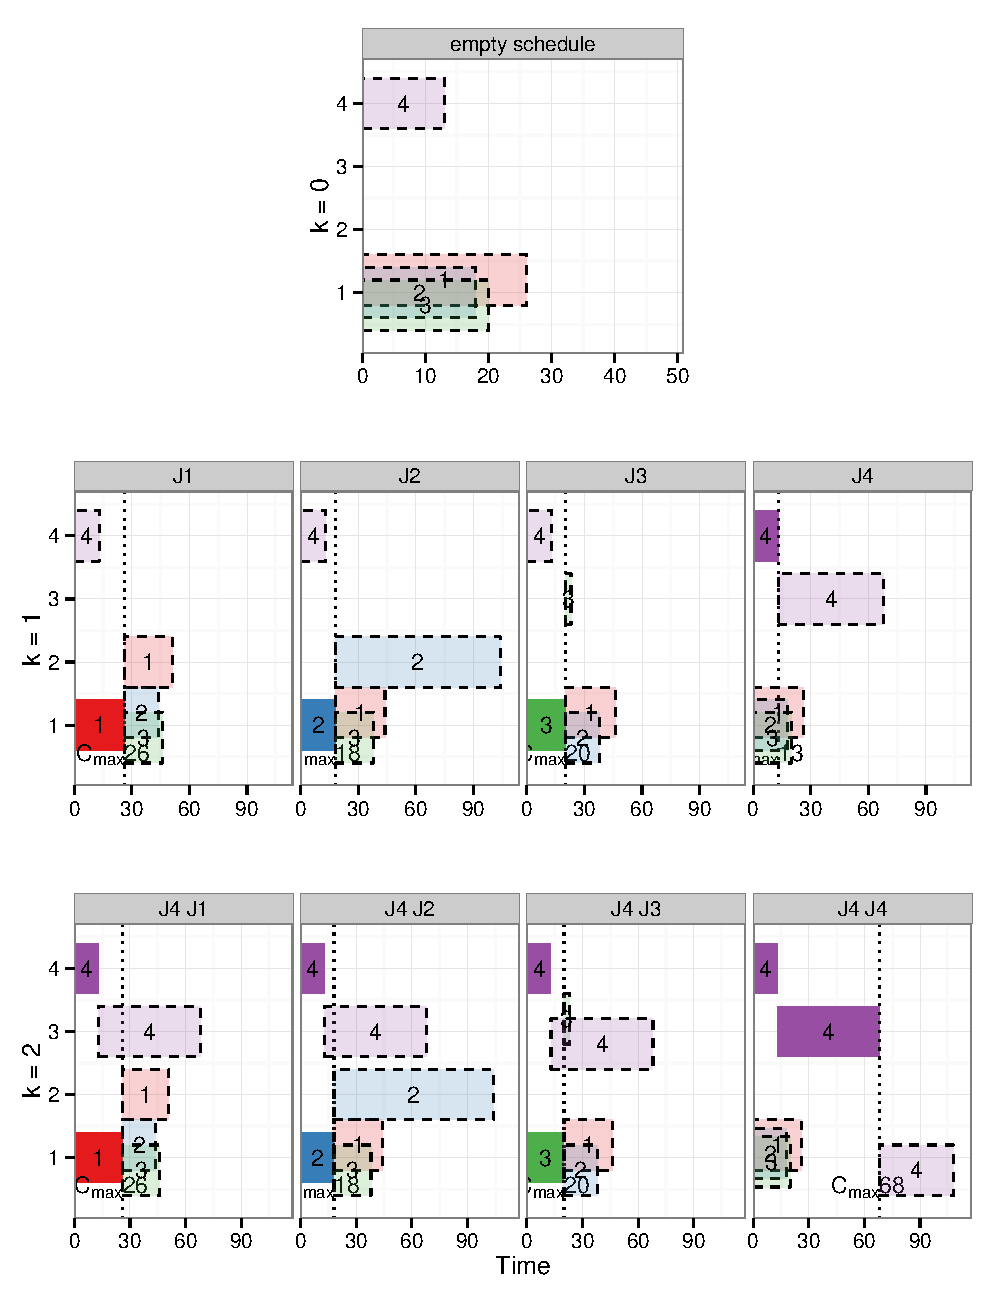
\includegraphics[width=\textwidth]{gametree}};
  \begin{scope}[x={(image.south east)},y={(image.north west)}]
  %% next four lines will help you to locate the point needed by forming a 
  %%grid. comment these four lines in the final picture.↓
  %\draw[help lines,xstep=.1,ystep=.1] (0,0) grid (1,1);
  %\draw[help lines,xstep=.05,ystep=.05] (0,0) grid (1,1);
  %\foreach \x in {0,1,...,9} { \node [anchor=north] at (\x/10,0) {0.\x}; }
  %\foreach \y in {0,1,...,9} { \node [anchor=east] at (0,\y/10) {0.\y};}
  %% upto here↑
  \node (J0) at (0.5,0.71) {};
  \node (J1) at (0.19,0.65) {};
  \node (J2) at (0.42,0.65) {};
  \node (J3) at (0.65,0.65) {};
  \node (J4) at (0.85,0.65) {};
  \draw[-latex] (J0) to[out=-20,in=+20] (J1);
  \draw[-latex] (J0) to[out=-20,in=+20] (J2);
  \draw[-latex] (J0) to[out=-20,in=+20] (J3);
  \draw[-latex] (J0) to[out=-20,in=+20] (J4);
  \node (J4) at (0.82,0.38) {};
  \node (J4J1) at (0.19,0.31) {};
  \node (J4J2) at (0.42,0.31) {};
  \node (J4J3) at (0.65,0.31) {};
  \node (J4J4) at (0.85,0.31) {};
  \draw[-latex] (J4) to[out=-20,in=+20] (J4J1);
  \draw[-latex] (J4) to[out=-20,in=+20] (J4J2);
  \draw[-latex] (J4) to[out=-20,in=+20] (J4J3);
  \draw[-latex] (J4) to[out=-20,in=+20] (J4J4);
  \end{scope}
  \end{tikzpicture}

  \vspace{-27pt}
  \caption[Partial Game Tree for \jsp]{Partial Game Tree for \jsp\ for the 
    first two dispatches. 
    Top layer depicts all possible dispatches (dashed) for an empty schedule. 
    Middle layer depicts all possible dispatches given that one of the 
    dispatches from the layer above has been executed (solid). 
    Bottom layer depicts when job $J_4$ on machine $M_4$ has been chosen to be 
    dispatched from the previous layer, moreover it depicts all possible next 
    dispatches from that scenario.}
  \label{fig:jssp:gametree}
\end{figure}

\subsection{Labelling schedules w.r.t. optimal 
decisions}\label{sec:gentrdat:labelling}